\chapter{Réalisation}
  Ce chapitre présente plusieurs implémentations effectuées avec différentes
  technologies. Ces technologies sont :
  \begin{itemize}
    \item \emph{Dart},
    \item \emph{HTML5} $+$ \emph{Javascript}
    \item \emph{Java} \emph{GWT}
  \end{itemize}
  Chacune de ces implémentations partagent une partie commune, celle de la
  communication, qui utilise des servlets\footnote{classe \emph{Java} exécutée
  dynamiquement dans un serveur Web, étendant ainsi ses fonctionnalités} et
  \emph{Jxta} pour mettre en place le réseau Pair-à-Pair.

  \section{Implémentation en \emph{Dart}}
  \subsection{Qu'est-ce que \emph{Dart}}
  \subsection{Objectif de l'implémentation en \emph{Dart}}
  \subsection{État d'avancement}



  \section{Implémentation en \emph{HTML5} avec \emph{Javascript}}
	\label{sec:html5}
  \subsection{Qu'est-ce que \emph{HTML5}}
  
	\emph{HTML} (HyperText Markup Language) est le format de données conçu pour 
	représenter les pages web. 

	\emph{HTML5} est la prochaine révision majeure d'\emph{HTML}. 
	Cette nouvelle version d'\emph{HTML5} est encore est en cours de 
	développement et apporte un grand nombre d'améliorations.
	De nouvelles balises, de nouveaux attributs, une plus grande rapidité et des
	évolutions importantes comme les \emph{Web Workers} et les \emph{Events}.
	
	Les \emph{Web Workers} vont permettre de passer outre la limitation 
	historique de Javascript à ne pas supporter les multi-thread.
	Les APIs des \emph{Web Workers} définissent justement un moyen d’exécuter 
	des scripts en tâche de fond. Cela va donc permettre d’exécuter des 
	traitements sur des threads séparés vivant à côté de la page principale et 
	n’ayant pas d’impact sur ses performances d’affichage. 
	
	Les \emph{Server Sent Events} vont permettre d'envoyer des évènements du 
	serveur vers le client, tandis que les \emph{DOM}
	\footnote{Domain Object Model} \emph{Events} vont quand à eux	permettre 
	d'ajouter des évènements à chaque élément d'une page web.
	
	\subsection{Objectif de l'implémentation en \emph{HTML5} avec
		\emph{Javascript}}
	
	L'implémentation avec \emph{Javascript} et \emph{HTML5} permet de réunir 
	l'interface graphique et le modèle du logoot dans un même composant, et non de
	devoir les séparer en deux composants comme en \emph{GWT} \ref{gwt}, tout en gagnant énormément en rapidité et efficacité.
	
	L'éditeur de texte est une balise éditable grâce à la propriété 
	\emph{contenteditable} et les évènements vont pouvoir être récupérés et 
	ré-implémentés à notre bon vouloir.
	
	\subsection{État d'avancement}

	Pour implémenter notre éditeur, on utilise donc une \emph{div} qui n'est pas
	un élément très contraignant, ce qui permet de récupérer la position du
	curseur de façon assez simple et de parcourir les enfants représentant 
	chaque caractère par des \emph{span} grâces aux méthodes de parcours des 
	éléments du DOM, comme \emph{previousSibbling} ou \emph{parentNode} par 
	exemple.
	
	Concrétement, voilà les fonctionnalités proposés par cette version :
	\begin{itemize}
		\item Insertion et suppression de caractères
		\item Différenciation des clients via couleurs différentes 
	\end{itemize}
	
	L'insertion de caractères va être récupéré et modifié de façon à créer une 
	balise \emph{span} à chaque insertion, contenant en identifiant l'id généré 
	par l'algorithme du logoot, permettant de trier le texte, et d'insérer les 
	caractères directement au bon endroit sans avoir à passer par le calcul des 
	différences pour détecter les modifications éffectués.
	De plus, cela permet d'assigner une couleur à chaque utilisateur 
	en rajoutant un style spécifique à chaque \emph{span} en fonction du
	replica unique à chaque client.

	\begin{figure}[h]
		\label{fig:html5}
		
\includegraphics[width=\textwidth]{includes/html5.png}
		\caption{Ajout d'un caractère via l'éditeur \emph{HTML5}}
	\end{figure}
	
	Lors de la suppression, l'évènement est lui aussi récupéré et l'on peut 
	récupèrer directement le \emph{span} supprimer grâce à la position du curseur
	du client, ce qui rend la	suppression très simple, sans avoir à effectuer une
	différence pour trouver les changements effectués.
		
	Pour finir, il reste encore quelques améliorations et finition à porter sur 
	la version \emph{HTML5} du projet :
	\begin{itemize}
		\item Retour à la ligne
		\item Affichage du curseur des différents clients
		\item Suppression multiple de caractères
		\item Copier/coller de caractères
	\end{itemize}
	
	Ces améliorations ne sont pas impossible à rajouter et pourraient être 
	implémentées dans une version future.
	
	Le retour à la ligne doit être représenté avec la balise spécifique 
	\emph{<BR/>} ce qui posait quelques problèmes dans le parcours des éléments du
	DOM lorsque l'on récupérait le parent et les frères suivants des éléments.
	
	L'affichage des curseurs des différents clients s'apparente un peu au problème
	des retours à la ligne dans le sens ou la fonction est prévue en \emph{HTML5} 
	mais est représenté lui aussi par une balise spécifique ce qui imposerait de 
	faire des cas spécifiques en fonction de la valeur du \emph{span} qui 
	pourrait donc contenir soit un caractère soit une balise \emph{HTML}.
	
	La suppression multiple de caractère impose seulement de traiter 
	l'insertion en fonction de la taille de la sélection du curseur, et dans le 
	cas ou la sélection n'est pas vide, traiter l'évènement de manière différente.
	
	De même que la suppression, le copier/coller peut être récupéré via un 
	évènement \emph{HTML5} pré-définis et demanderait donc d'être traité de 
	manière différente que l'insertion d'un simple caractère.
	selection


  \section{Implémentation en \emph{Java} \emph{GWT}}
  \label{sec:gwt}
  \subsection{Qu'est-ce que \emph{GWT}}
  Google Web Toolkit est un ensemble d'outils fournis par Google pour le
   développement d'application web complexe. C'est un \emph{framework} gratuit
   et open source.
   
   Lors du développement, le code est écrit en  \emph{Java}. Ensuite \emph{GWT} 
   inclus un compilateur qui le traduit en \emph{Javascript} afin de le rendre 
   compatible avec tous les navigateur du marché.
   
  \subsection{Objectif de l'implémentation en \emph{Java} \emph{GWT}}
  L'avantage d'utiliser \emph{GWT} est la possibilité de decouper notre 
  logiciel de facon complétement modulaire. En effet, nous respectons la
  conception du chapitre précédent \ref{chap:Conception}. Grâce à cela, 
  l'interface utilisateur, la gestion du réseau et le moteur \emph{logoot}
  sont totalement découplés les uns des autres. L'objectif de départ étant
  de fournir deux interfaces : une en client leger (web avec \emph{Javascript})
  et une en client lourd (avec \emph{Swing}\footnote{Swing est une bibliothèque
  graphique pour \emph{Java}}). 
  
  \subsection{État d'avancement}
	L'implentation est complétement fonctionnel mais nous nous sommes heurtés
	à de nombreux problèmes.
	
	\label{sec:textarea}
	Pour implémenter l'éditeur, on utilise un \emph{TextArea}. C'est le 
	composant de base en \emph{html} pour ce genre de tâches. Cet élément 
	est trés contraignant. En effet la gestion du curseur est complexe
	pour des raisons de sécurité (afin d'éviter une intrusion trop forte côté 
	client). Afin de changer le texte quand des changement sont effectué à 
	l'exterieur, il redéfinir le texte entiérement après un 
	passage dans un algorithme de \emph{diff}\footnote{permet la comparaison 
	de texte en trouvant les différences}/\emph{patch}\footnote{integration
	d'un resultat de diff pour introduire les modifications}. Ce procédé
	est lent et a tendance à nous faire perdre certains caractères lorsque
	l'on tape rapidement.
	
	Le protocol clasique de communication utilisé sur le web n'est pas 
	adapté à notre projet. En général, ce sont les pages web qui requêtent
	le serveur et celui-ci réponds. Aucun problème pour envoyer nos modifications 
	au serveur via un appel RPC fournis par \emph{GWT}. Le problème se présente
	pour permettre la réception des modifications. Plusieurs solutions 
	techniques sont disponible :
	\begin{itemize}
		\item \emph{Server Push} : La méthode consiste à ne pas clore la
		transaction coté serveur. Aprés une requête du client, le serveur
		répond quand il le souhaite. Afin de permetre une connection continue 
		entre le client et le serveur, le client doit à la réception d'une 
		réponse émettre une nouvelle requête.
		\item \emph{Web Socket}\cite{websocket_spec} : Il s'agit d'une spécification en cours au sein
		du \emph{WHATWG}\footnote{Web Hypertext Application Technology Working 
		Group} afin de permettre une communication bidirectionnel entre client
		et serveur. En raison de failles de sécurité et du coup d'implémentation 
		timide dans les navigateurs, nous n'avons pas retenu cette solution.
		\item \emph{Server Sent Event} \cite{server_sent_spec} 
		\cite{server_sent_html5_rocks} 
		 : Cette technologie est également en
		cours de spécification. Elle permet au client d'initier une connexion
		au serveur et de lui permettre d'envoyer les informations quand il
		le souhaite sans clore la connection.
	\end{itemize}
	
	Nous avons choisi d'utiliser les Server Sent Event pour leurs simplicités.
	Par contre, \emph{GWT} ne permet d'utiliser directement cette fonction.
	On utilise alors un mécanisme qui permet d'inclure du \emph{Javascript} natif.
	Là encore, on touche à la limite de ce que permet \emph{GWT}.

\section{Comparatif des implémentations}
\begin{table}[h!]
	\center
	\begin{tabular}{|l|c|c|c|} 
	\hline
	 ~ & \emph{Dart} & \emph{Javascript / HTML 5} & \emph{GWT}\\
	\hline
	Insertion unique & oui & oui &oui\\
	\hline
	Suppression unique & oui & oui & oui\\
	\hline
	Saut de ligne & oui & non & oui\\
	\hline
	Insertion bloc & oui & non & oui\\
	\hline
	Suppression bloc & oui & non & oui\\
	\hline
	Edition distante & non & oui & oui \\
	\hline
	Coloration & non & oui & non \\
	\hline
	Curseur statique\footnote{position du curseur cohérente lors de l'insertion d'un autre client} & non & oui & non \\ 
	\hline
	Curseur des clients & non & non & non \\
	\hline
	Performance & Moyenne & Bonne & Moyenne \\ 
	\hline
	\end{tabular}
\end{table}

  
  \section{Communication}
Les implémentations décrient précédemment utilisent une couche commune qui gère
la communication entre les différents utilisateurs d'un même document. Cette
couche est faite d'un serveur web offrant un service de connexion et un service
d'envoi / réception de message.

Le déploiement d'un nouveau serveur entraine la création d'un nouveau pair
dans l'essaim. Ainsi chaque nouveau serveur discute avec les autres serveurs
via un réseau pair-à-pair. 

En plus de la communication inter-serveur, chaque
serveur se comporte comme un point de connexion pour plusieurs client. Ainsi
un serveur est en charge de redistribué un messages à tous ses clients (via
un mécanisme interne de \emph{socket}) et aux autres serveurs du réseau (via
le réseau pair-à-pair).

Une telle configuration apporte des avantages certains :
\begin{enumerate}
 \item L'utilisation d'un réseau P2P accélère l'échange d'informations,
 améliore la sureté (meilleure tolérance au faute), ne pose pas de problème
 au niveau de la vie privée (\emph{Google Docs}) et s'accommode d'une demande
 de montée en charge ;
 \item L'utilisation du serveur comme point de communication permet une
 distribution simple de l'application (l'application est fournie par le
 serveur web).
\end{enumerate}

La figure \ref{fig:commu} page \pageref{fig:commu} présente la répartition des
pairs et des client. Un carré bleu est un serveur web et un pair. Un rond noir
est un client utilisant l'application.

\begin{figure}[hbt]
  \center
  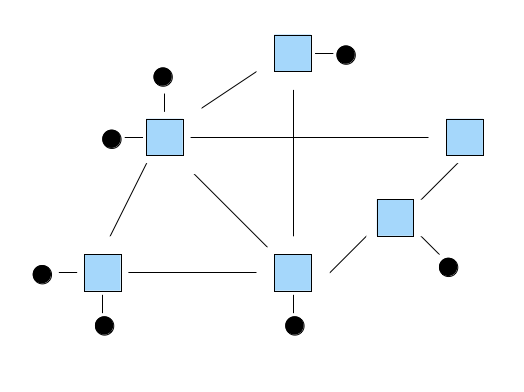
\includegraphics[width=.8\textwidth]{includes/network-model.png}
  \caption{Modèle de communication}
  \label{fig:commu}
\end{figure}



